After some tests with the earlier version of the software, some performance issues came to light. In particular the execution time was higher with more threads, the exact opposite of the expected behavior. After a deeper analysis of the execution I noted that the CPU was spending more time waiting for I/O from the disk than doing actual work (not very surprising given the well known limits of mechanical hard disks).\\
It became immediately clear that reading (and writing) only eight bytes at a time wasn't the best strategy, but on the other hand we could not even load the entire file in RAM (big files may saturate the RAM). So the best way to manage the problem in this case was to load a chunk of data to work on in a temporary buffer, do the encryption, and write out the result. I called these chunks of data \emph{frames}.

\begin{figure}[H]
\centering
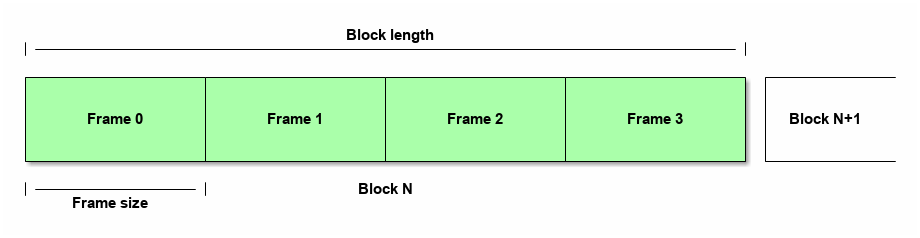
\includegraphics[scale = 0.4]{./Pictures/buffering} % x compreso tra 0 e 1
\caption{Buffering}
\label{fig:buffering}
\end{figure}

So now we have a second level of subdivision within every block, each block is subdivided in frames and only one frame per block (for each thread) is loaded in RAM. Once the work on the current frame is completed, the buffer is written out in the output file and the next frame is loaded. This time we don't have any problem of padding, because we simply divide the block size (which is already multiple of eight) by multiples of eight, so everything match and we don't have to worry about the reminder.\\
The frame size is determined dynamically at runtime because if the file to be encrypted is small there is no need to divide the blocks in frames, everything can be kept in RAM. To determine the frame size the algorithm compare the block size with a given threshold, if the block is smaller than the threshold we store the entire block in RAM, otherwise we divide it by eight and compare again, we keep dividing by multiple of eight until we reach a value lower than the threshold.\\
After some tests it turns out that the threshold value, over a certain point, doesn't affect the resulting performance and even a value small as 2MB allows the same performance as any higher value.\\
In the end this proves to be a very valid solution which lead to a big performance gain maintaining a low RAM usage.